\documentclass{article}

\usepackage{eikonal}

\begin{document}

\begin{figure}[h]
  \centering
  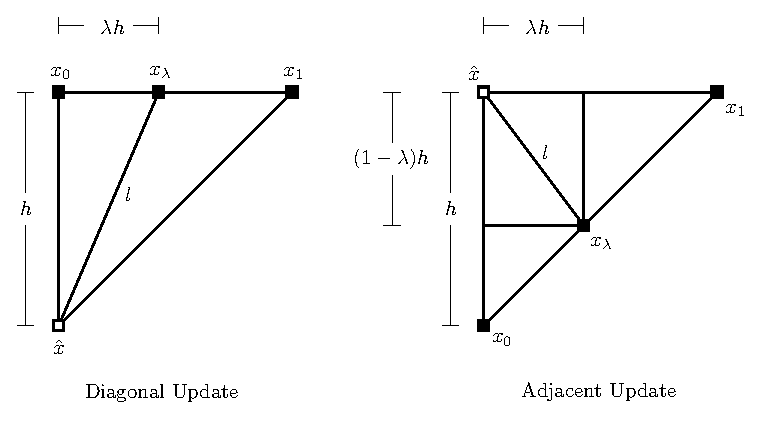
\includegraphics{computing-l.eps}
  \caption{Computing $l$ for each type of triangular update using $\lambda$ and the grid spacing $h$.}
  \label{fig:computing-l}
\end{figure}

\section{Righthand Rule}

In this document we will quickly derive the rule for each two-point
triangular update in the eight-point ordered line integral method
(OLIM) for solving $||\nabla u|| = s$. We denote each triangle's
vertices $\hat{x}, x_0$, and $x_1$, where $\hat{x}$ is the vertex
corresponding to the node whose value is to be updated. Then, with
$\hat{u} = u(\hat{x}), u_0 = u(x_0)$, and $u_1 = u(x_1)$, the general
update solves the following minimization problem, where $u$ is assumed
to be linear in the update triangle:
\begin{align*}
  \hat{u} := \min_{0 \leq \lambda \leq 1} \left\{ u_\lambda + \hat{s} ||\hat{x} - x_\lambda||\right\},
\end{align*}
where $\hat{s} = s(\hat{x})$, $x_\lambda = (1 - \lambda) x_0 + \lambda x_1$, and
$u_\lambda = u(x_\lambda) = (1 - \lambda)u_0 + \lambda u_1$.

There are two types of two-point updates, which we refer to as
``adjacent'' and ``diagonal'' updates. In adjacent updates, both $x_0$
and $x_1$ are directly adjacent to $\hat{x}$; in diagonal updates,
exactly one of $x_0$ or $x_1$ is diagonally adjacent to $\hat{x}$. In
what follows, we let $\alpha = |u_1 - u_0|/(\hat{s} h)$.

\begin{lemma}\label{lemma:rhr-diagonal-update}
  For the diagonal update, the minimizing $\lambda^*$ is given by
  $\lambda^* = \alpha/\sqrt{1 - \alpha^2}$.
\end{lemma}

\begin{proof}
  Since $u$ is assumed to be linear in the update triangle, we have
  $\hat{u} = (1 - \lambda) u_0 + \lambda u_1 + \hat{s} ||\hat{x} -
  x_\lambda||$. From Figure~\ref{fig:computing-l}, it's clear that
  $l = ||\hat{x} - x_\lambda|| = h \sqrt{\lambda^2 + 1}$. Then:
  \begin{align*}
    0 = \frac{d \hat{u}}{d \lambda} = -u_0 + u_1 + \frac{\hat{s} h \lambda}{\sqrt{\lambda^2 + 1}} \implies \alpha^2 = \frac{\lambda^2}{\lambda^2 + 1} \implies \lambda = \frac{\alpha}{\sqrt{1 - \alpha^2}}.
  \end{align*}
  In the last step, we have chosen $\lambda$ to be the positive root
  of the radical, since $\lambda$ is a convex coefficient and a
  negative value would be nonsensical.
\end{proof}

\begin{lemma}\label{lemma:rhr-adjacent-update}
  For the adjacent update, $\lambda^*$ satisfies:
  \begin{align*}
    \lambda^* = \frac{1}{2} \pm \frac{\sqrt{3} \alpha}{2 \sqrt{\alpha^2 + 2}}.
  \end{align*}
\end{lemma}

\begin{proof}
  The previous proof goes through essentially as before, but with the
  modification that the value $l = ||\hat{x} - x_\lambda||$ is instead
  given by $l = h \sqrt{\lambda^2 + (1 - \lambda)^2}$.
\end{proof}

We note that if $x_0$ and $x_1$ are swapped in the diagonal update,
the value for $\lambda^*$ changes, and is \emph{slightly} more
expensive to compute. It is possible to compute all eight diagonal
updates using Lemma 1, but care must be taken to ensure that the nodes
neighboring $\hat{x}$ are labeled properly.

\section{Midpoint Rule}

\begin{figure}[h]
  \centering
  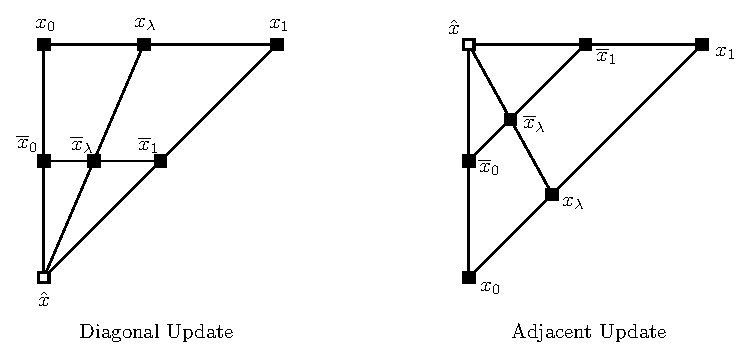
\includegraphics{midpoint_update.eps}
  \caption{The arrangement of points for the two point updates in the
    midpoint rules.}\label{fig:midpoint-update}
\end{figure}

To approximate $\hat{u}$ with a higher order integration scheme, we
additionally consider the points
$\overline{x}_0 = (x_0 + \hat{x})/2, \overline{x}_1 = (x_1 +
\hat{x})/2$, and $(x_\lambda + \hat{x})/2$. As before, we use the
simplified notation
$\overline{u}_0 = u(\overline{x}_0), \overline{u}_1 =
u(\overline{x}_1)$, and so on. The speed function $s$ presents some
complication: to avoid evaluating its derivative, we consider zeroth
and first order approximations to it at the point
$\overline{x}_\lambda$. These two approximations will yield our two
midpoint updates. In both cases, we start by approximating:
\begin{align*}
  u_{\lambda} + \int_0^{||\hat{x} - x_\lambda||} s(t) dt = u_\lambda + \overline{s}_\lambda ||\hat{x} - x_\lambda|| + \epsilon.
\end{align*}
For constant approximation, we take
$\overline{s}_\lambda = (\overline{x}_0 + \overline{x}_1)/2$; for the
first order approximation,
$\overline{s}_\lambda = (1 - \lambda) \overline{x}_0 + \lambda
\overline{x}_1$. As before, to compute $||\hat{x} - x_\lambda||$, we
use Figure~\ref{fig:computing-l}.

\subsection{Constant Approximation}

For the constant approximation, we can simply replace $\hat{s}$ in
Lemmas~\ref{lemma:rhr-diagonal-update}
and~\ref{lemma:rhr-adjacent-update} with $\overline{s}_\lambda$. Then,
the algorithm for the righthand rule derived in the preceding section
will apply to the midpoint rule with constant approximation to
$\overline{s}_\lambda$.

\subsection{Linear Approximation}

For the linear approximation, we proceed in a similar way to the
previous section; however, in this case, we find that $\lambda$
corresponds to the roots of a quartic equation.

\begin{lemma}\label{lemma:midpoint-diagonal-update}
  Let $\alpha = |u_0 - u_1|/h$ and
  $\delta \overline{s} = \overline{s}_1 - \overline{s}_0$. Then, for
  the diagonal triangular update, $\lambda$ can be found from the
  roots of the quartic:
  \begin{align*}
    p(\lambda) = 4 \delta \overline{s} \lambda^4 + 4 \overline{s}_0 \delta \overline{s} \lambda^3 + {(4 \delta \overline{s} + \overline{s}_0^2 - \alpha^2)} \lambda^2 + 2 \overline{s}_0 \delta \overline{s} \lambda + \delta \overline{s} - \alpha^2.
  \end{align*}
\end{lemma}

\begin{proof}
  We define
  $g(\lambda) = u_\lambda + \overline{s}_\lambda h \sqrt{1 +
    \lambda^2}$. Then, letting
  $\delta \overline{s} = \overline{s}_1 - \overline{s}_0$, we have:
  \begin{align*}
    g'(\lambda) = -u_0 + u_1 + h \frac{\partial}{\partial \lambda} \left\{\left(\overline{s}_0 + \lambda \delta \overline{s}\right) \sqrt{1 + \lambda^2}\right\}
  \end{align*}
  so that setting $g'(\lambda) = 0$ gives us:
  \begin{align*}
    \frac{u_0 - u_1}{h} &= \frac{\overline{s}_0 \lambda}{\sqrt{1 + \lambda^2}} + \delta \overline{s} \left(\frac{\lambda^2}{\sqrt{1 + \lambda^2}} + \sqrt{1 + \lambda^2}\right).
  \end{align*}
  Multiplying through by $\sqrt{1 + \lambda^2}$ and squaring boths
  sides gives:
  \begin{align*}
    {(1 + \lambda^2)} \alpha^2 = \overline{s}_0^2 \lambda^2 + 2 \overline{s}_0 \delta \overline{s} \lambda {(1 + 2\lambda^2)} + \delta \overline{s} {(1 + 2\lambda^2)}^2.
  \end{align*}
  Collecting terms, and defining $p(\lambda)$ to be the resulting
  polynomial gives us the result.
\end{proof}

\begin{lemma}\label{lemma:midpoint-adjacent-update}
  Let $\alpha$ and $\delta \overline{s}$ be defined as in
  Lemma~\ref{lemma:midpoint-diagonal-update}. For the adjacent
  triangular update, $\lambda$ can be found from the roots of:
  \begin{align*}
    p(\lambda) = 16 \delta \overline{s}^2 \lambda^4 - 8 {(3 \delta \overline{s}^2 - 2 \overline{s}_0 \delta \overline{s})} \lambda^3 + {(17 \delta \overline{s}^2 - 20 \overline{s}_0 \delta \overline{s} + 4 \overline{s}_0^2 - 2 \alpha^2)} \lambda^2 - 2 {(3 \delta \overline{s}^2 + 5 \overline{s}_0 \delta \overline{s} - 2 \overline{s}_0^2 + \alpha^2)} \lambda + {(\overline{s}_0 - \delta \overline{s})}^2 - \alpha^2.
  \end{align*}
\end{lemma}

\begin{proof}
  Proceeding similarly, we now define
  $g(\lambda) = \hat{u} + \overline{s}_\lambda h \sqrt{2 \lambda^2 -
    2\lambda + 1}$. Then:
  \begin{align*}
    g'(\lambda) = -u_0 + u_1 + h \left[\frac{2\lambda - 1}{\sqrt{2\lambda^2 - 2\lambda + 1}} \overline{s}_0 + \left(\sqrt{2\lambda^2 - 2\lambda + 1} + \frac{2\lambda^2 - \lambda}{\sqrt{2\lambda^2 - 2\lambda + 1}}\right)\delta \overline{s}\right].
  \end{align*}
  Setting $g'(\lambda)$ equal to zero, multiplying by
  $\sqrt{2\lambda^2 - 2\lambda +1}$, and simplifying, we obtain:
  \begin{align*}
    \frac{u_0 - u_1}{h} \sqrt{2\lambda^2 - 2\lambda + 1} = {(2\lambda - 1)}\overline{s}_0 + {(4\lambda^2 - 3\lambda + 1)} \delta \overline{s}.
  \end{align*}
  Finally, we square both sides, collect like terms, and define
  $p(\lambda)$ from the resulting quartic in $\lambda$.
\end{proof}

\begin{note}
  When $s \equiv 1$, then the midpoint rule offers no advantage beyond
  the right-hand rule. Observe that $s \equiv 1$ implies
  $\delta \overline{s} = 0$, which reduces $p$ in
  Lemma~\ref{lemma:midpoint-diagonal-update} to
  $p(\lambda) = (1 - \alpha^2) \lambda^2 + \alpha^2$. 
\end{note}

\end{document}

%%% Local Variables:
%%% mode: latex
%%% TeX-master: t
%%% End:
